% !TEX encoding = UTF-8
% !TEX TS-program = pdflatex
% !TEX root = ../thesis.tex

%**************************************************************
\chapter{METODOLOGIA}
\label{Capitolo3}
\thispagestyle{empty}

Nel capitolo precedente sono stati spiegati tutti i concetti principali che 
compongono un sistema di visione artificiale, il quale ha lo scopo fondamentale 
di effettuare la comprensione della scena mediante l'utilizzo di tecniche 
di object detection e di semantic segmentation. Avendo come obiettivo 
principale lo sviluppo di un sistema di guida autonoma, nel seguente capitolo 
vengono riportate tutte le metodologie utilizzate per tale scopo. Il focus 
principale sarà rivolto verso la tecnica di segmentazione semantica. È 
proprio quest'ultima tecnica quella ad essere utilizzata maggiormente in 
questo elaborato. Le risorse computazionali richieste da codesta risultano 
essere onerose. Essendo un sistema autonomo implementato all'interno di 
una centralina dedicata, bisogna aver un chiaro prospetto delle potenzialità 
richieste da un modello di visione artificiale, affinché si raggiunga l'obiettivo 
finale. Uno degli obiettivi di questo elaborato è basato sull'implementazione 
di metodi di guida autonoma su un dispositivo, relativamente economico, 
alla portata di tutti. La centralina presa di riferimento è rappresentata da 
un nota scheda di elaborazione embedded, che prende il nome di Jetson 
Nano (NVidia). Le potenzialità messe a disposizione da questa scheda sono 
state comparate, in termini di Frames-per-Second (FPS), con quelle messe 
a disposizione sia dal computer del sottoscritto che da Google Colaboratory 
(Colab). Avendo caratteristiche hardware ben differenti l'uno dall'altro, si è 
pensato di creare una comparazione standard composta dallo stesso codice 
eseguito su tutte e tre le diverse architetture. Per la visualizzazione dei 
risultati ottenuti in ogni test, si rimanda la lettura al capitolo (\ref{Chapter4}).

\section{Jetson Nano}
La Jetson Nano (B01), presentata nel Marzo del 2019,  è una scheda embedded 
sviluppata da NVidia che rappresenta il prodotto più piccolo della 
famiglia Jetson. L'utilizzo della scheda è rivolto principalmente verso varie 
applicazioni di intelligenza artificiale, visione artificiale e robotica. A bordo 
troviamo un processore e una scheda madre che offre una potenza di calcolo 
pari a 128 Cuda cores. L'obiettivo di questa scheda è quello di funzionare 
con reti neurali e offrire le migliori prestazioni quando viene utilizzata per 
eseguire inferenze. A differenza di altre architetture, lo Jetson Nano utilizza 
una precisione a 16-bit che lo rende competitivo rispetto ad altri device 
embedded. Purtroppo non supporta la precisione a 8-bit ma è comunque in 
grado di lavorare con qualsiasi rete disponibile e con qualsiasi framework di 
deep learning popolare (es: Pytorch, TensorFlow, Keras, Caffe etc.). In questo 
dispositivo è possibile effettuare sia il rilascio (deploy) dell'applicazione 
che l'addestramento della rete ma, in quest'ultimo caso, risulta essere lento 
a causa delle prestazioni computazionali ridotte. Oltre ad avere il vantaggio 
delle dimensioni ridotte, un altro principale vantaggio dello Jetson Nano 
deriva dall'applicazione dell'ottimizzazione TensorRT. Quest'ultima esegue 
un processo di quantizzazione che è utile a convertire i pesi e gli input in 
tipi interi, in modo da preservare la memoria che, su una scheda del genere, 
rappresenta una limitazione. A tal proposito, il dispositivo non fornisce 
alcun tipo di memoria integrata, ma esiste la possibilità di aggiungerne una 
grazie alla presenza di uno slot di espansione in cui è possibile alloggiare 
una scheda micro-sd. Essendo una scheda embedded, a differenza di altri 
computer che utilizzano alimentatori da diversi Watts (W), il Jetson Nano 
può utilizzare due diversi livelli di wattaggio. Il primo, quello da 5W, è 
raggiungibile grazie alla presenza di una porta micro-usb, mentre il secondo, 
quello da 10W, è raggiungibile solo grazie all'utilizzo di un alimentatore 
esterno collegato all'ingresso jack. Il massimo livello di performance, raggiungibile 
dalla GPU, avviene tramite l'utilizzo dell'alimentatore esterno. 
Per rendere l'idea delle dimensioni e dell'intera architettura, in Figura (\ref{jetson}) 
è riportata la Jetson Nano.
\begin{figure}[]
    \begin{minipage}[t]{.45\textwidth}
        \centering
        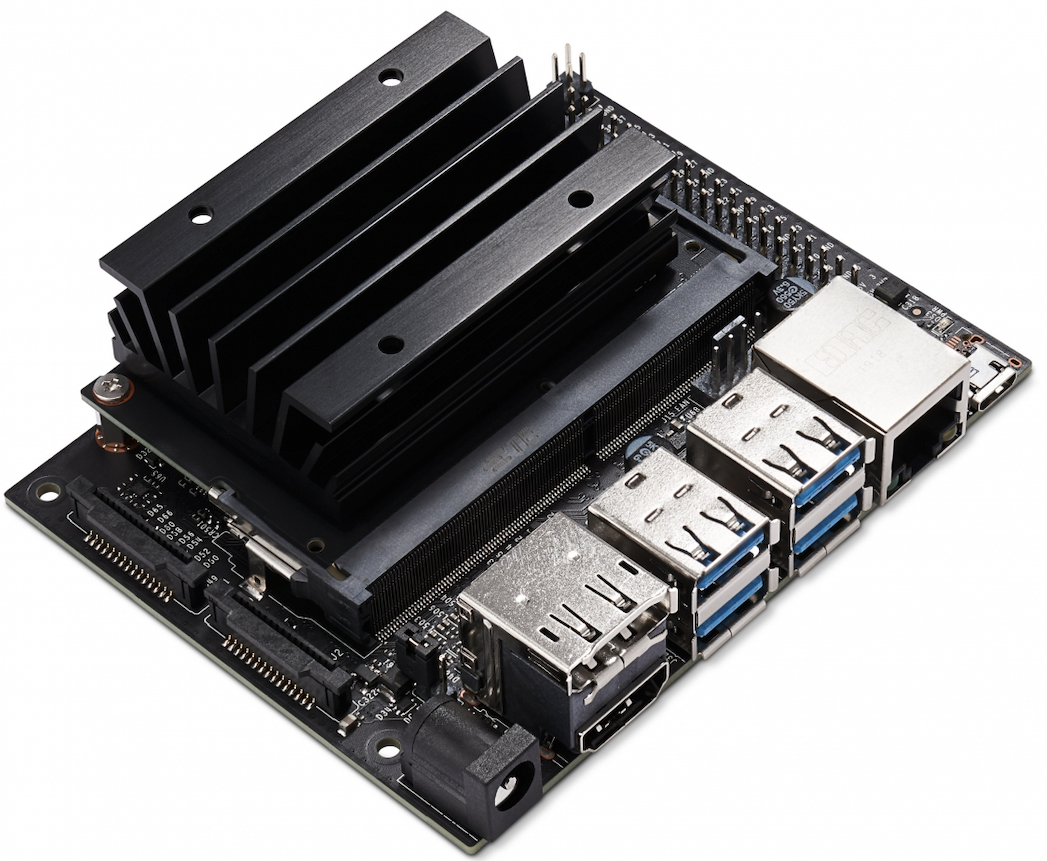
\includegraphics[width=\textwidth]{jetson1.png}
    \end{minipage}
    \hfill
    \begin{minipage}[t]{.45\textwidth}
        \centering
        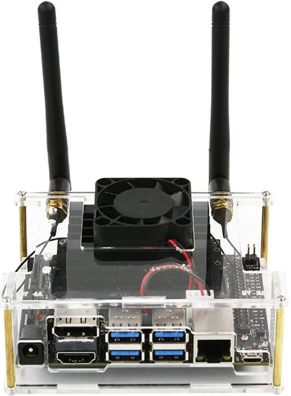
\includegraphics[width= 0.8\textwidth]{jetson2.png}
    \end{minipage}  
    \caption{NVidia Jetson Nano.}
    \label{jetson}
\end{figure}

\section{TensorRT}
\begin{figure}
    \centering
    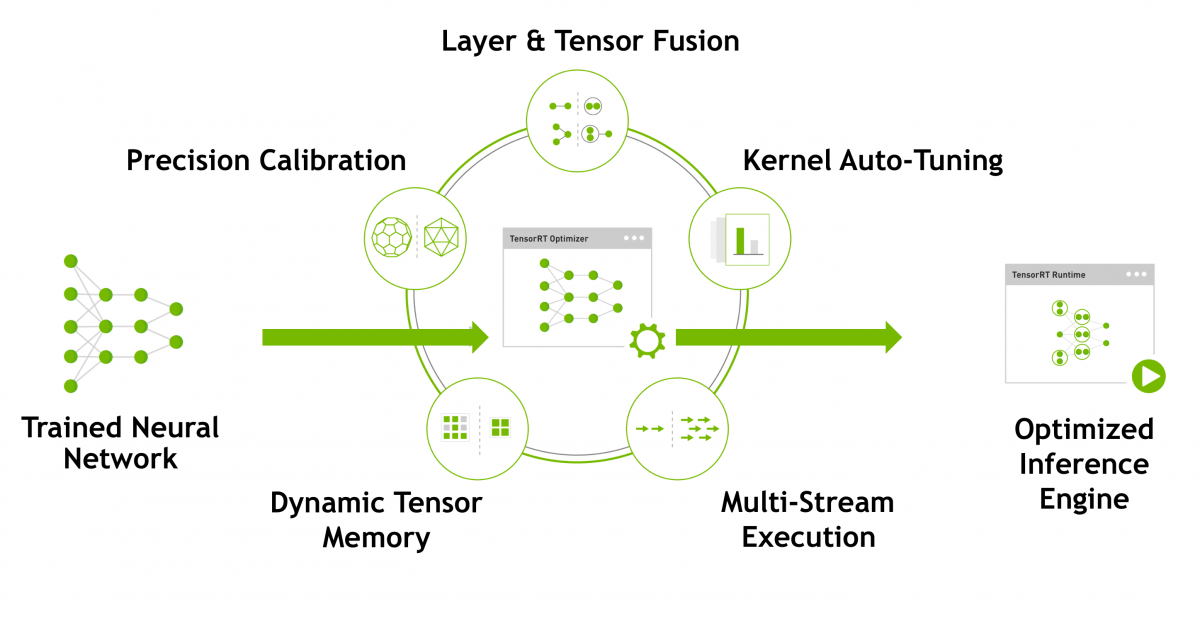
\includegraphics[width = \linewidth]{tensorrtOpt.png}
    \centering
    \caption{Ottimizzazioni si TensorRT sui modelli.}
    \label{tensorrt}
\end{figure}
TensorRT è un framework di machine learning, sviluppato interamente da 
NVidia, che esegue cinque diverse procedure di ottimizzazione su architetture 
basate su scheda GPU NVidia (Fig. (\ref{tensorrt})). 
\begin{enumerate}
    \item {\bfseries{\emph{Precision Calibration}}}: in questa ottimizzazione viene eseguita 
    l'operazione di \emph{Quantizzazione} che permette di mappare tutti i valori 
    dei pesi da una precisione FP32 bit a FP16 bit, creando una perdita 
    di precisione trascurabile.
    \item {\bfseries{\emph{Layer \& Tensor Fusion}}}: la seconda ottimizzazione riguarda l'eliminazione 
    di tutti quei layer che non vengono utilizzati, questo è 
    utile per poter evitare calcoli inutili. Successivamente, le operazioni 
    di Convoluzione, ReLU e normalizzazione Batch, vengono fuse in un 
    unico layer (\emph{CBR}). Questa operazione permette di eseguire calcoli 
    in una maniera più veloce ed efficace. Nella Figura (\ref{fusion_tensorrt}) si possono 
    vedere meglio quali sono tutti i layer che vengono fusi da TensorRT.
    \item {\bfseries{\emph{Kernel Auto-Tuning}}}: la terza ottimizzazione viene effettuata direttamente 
    sui filtri utilizzati nella rete. Durante questa fase vengono 
    selezionati i migliori layer, algoritmi e dimensioni di batch in base alla 
    piattaforma GPU di destinazione.
    \item {\bfseries{\emph{Dynamic Tensor Memory}}}: la gestione della memoria viene effettuata 
    proprio in questa ottimizzazione. TensorRT alloca memoria 
    solo per durante il periodo di vita di un tensore scongiurando un 
    sovraccarico di allocazioni permettendo esecuzioni rapide ed efficienti.
    \item {\bfseries{\emph{Multiple Stream Execution}}}: l'ultima ottimizzazione riguarda l'elaborazione 
    parallela di multipli flussi di input. Fondamentalmente, 
    questo è possibile utilizzando la libreria CUDA stream.
\end{enumerate}
L'aspetto più importante da ricordarsi, quando si utilizza TensorRT, è che 
bisogna assicurarsi che la procedura di ottimizzazione avvenga sulla stessa 
GPU NVidia che verrà utilizzata per l'inferenza. Questo deve avvenire 
in quanto TensorRT utilizza kernel specifici a seconda della piattaforma 
di destinazione. L'utilizzo di una ottimizzazione su una differente scheda 
grafica porta alla creazione di errori in fase di inferenza. 
\begin{figure}
    \centering
    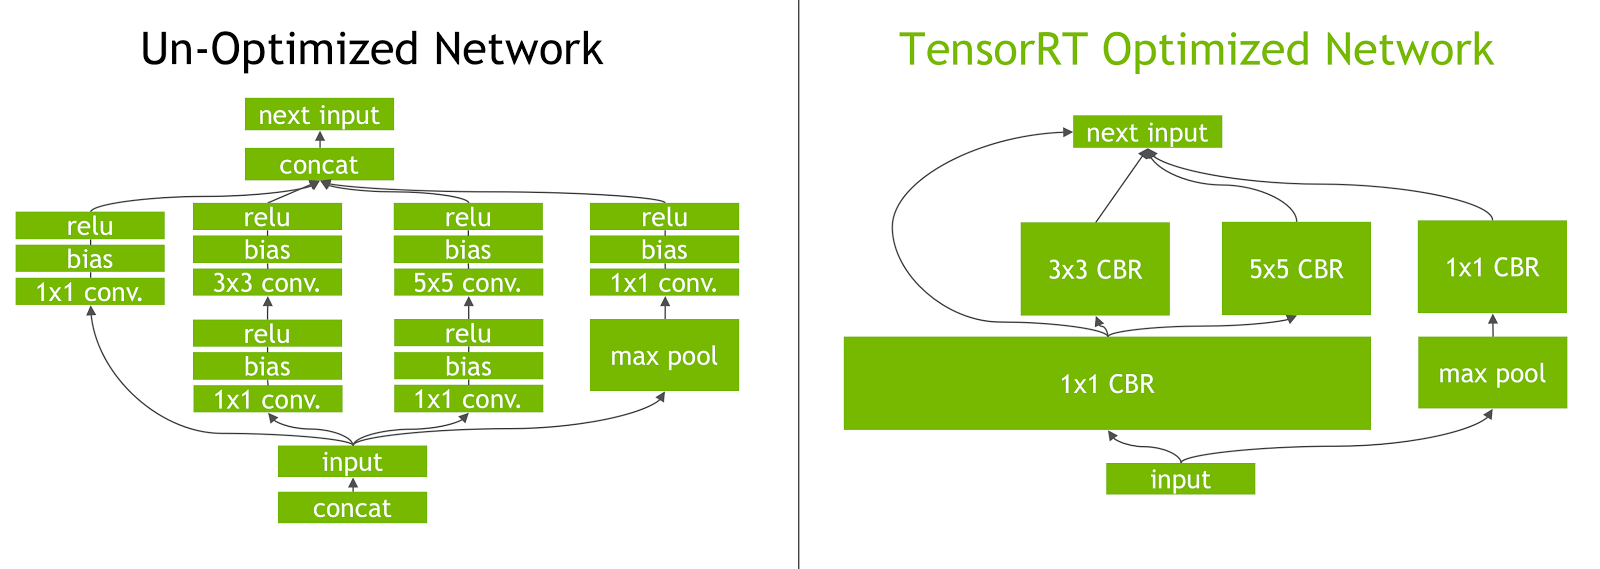
\includegraphics[width = \linewidth]{optTensor.png}
    \centering
    \caption{Fusione dei livelli Convolutional, Batch e ReLU eseguita da TensorRT.}
    \label{fusion_tensorrt}
\end{figure}



\section{Frames-per-Second (FPS)}
La velocità di inferenza rappresenta un indicatore di performance di ogni 
modello. Per poterla calcolare, la velocità di inferenza è rappresentata dai 
\emph{Frames-per-Second (FPS)} (\ref{FPS_Count}):
\begin{equation}\label{FPS_Count}
    FPS = \frac{1}{Ending \ Time - Starting \ Time}
\end{equation}
Questa misura è variabile e serve per rappresentare tre diversi elementi:
\begin{itemize}
    \item {\bfseries{\emph{Input}}}: ogni rete prende in input una sequenza di frame appartenenti 
    a un video. Ogni video può avere un numero di FPS variabile. In 
    questo elaborato, vengono testati diversi video a 30FPS e a 60FPS.
    \item {\bfseries{\emph{Netwrok}}}: la velocità che la rete impiega ad effettuare uno specifico 
    task, può essere rappresentata dal numero di FPS. Riconoscere e/o 
    segmentare un oggetto appare essere un'attività onerosa in termini 
    computazionali, pertanto una rete è considerata veloce se, oltre a 
    produrre un output adeguato, svolge ogni task in un tempo breve.
    \item {\bfseries{\emph{Output}}}: il risultato prodotto da una rete è visibile solamente a 
    schermo. Il video mostrato ha anch'esso una velocità di riproduzione 
    che è influenzato dal numero di FPS.
\end{itemize}